\documentclass[a4paper,10pt]{article}

% --- TIMES NEW ROMAN & ATS ENCODING ---
\usepackage[T1]{fontenc}
\usepackage{times}

\usepackage[a4paper,margin=0.40in]{geometry}
\usepackage{enumitem}
\usepackage{titlesec}
\usepackage[hidelinks]{hyperref}
\usepackage{graphicx}

% Clean, tight spacing for section headings
\titleformat{\section}{\large\bfseries}{}{0em}{}[\titlerule]
\titlespacing*{\section}{0pt}{5pt}{4pt}

% Globally reduce itemize vertical heights (pointers height reduction)
\setlist[itemize]{
    noitemsep,
    topsep=1pt,
    parsep=0pt,
    partopsep=0pt,
    itemsep=1.5pt
}

\setlength{\parindent}{0pt}

\begin{document}
\pagestyle{empty}

% HEADER
\begin{minipage}[t]{0.75\textwidth}
    {\LARGE \textbf{SHIV SANTOSH SARWADE}}\\[4pt]
    {\Large \textbf{Software Developer}}\\[6pt]
    \textbf{Phone:} +91-7620876612\\
    \textbf{Email:} \href{mailto:shiv.s.sarwade@gmail.com}{shiv.s.sarwade@gmail.com}\\[4pt]
    \textbf{Links \& Profiles:}\\
    \href{https://shivsarwade.vercel.app/}{shivsarwade.vercel.app} (Portfolio)\\
    \href{https://linkedin.com/in/shiv-sarwade}{linkedin.com/in/shiv-sarwade} (LinkedIn)\\
    \href{https://github.com/ShivSarwade}{github.com/ShivSarwade} (GitHub)\\
\end{minipage}%
\begin{minipage}[t]{0.25\textwidth}
    \vspace{-10pt}
    \raggedleft
    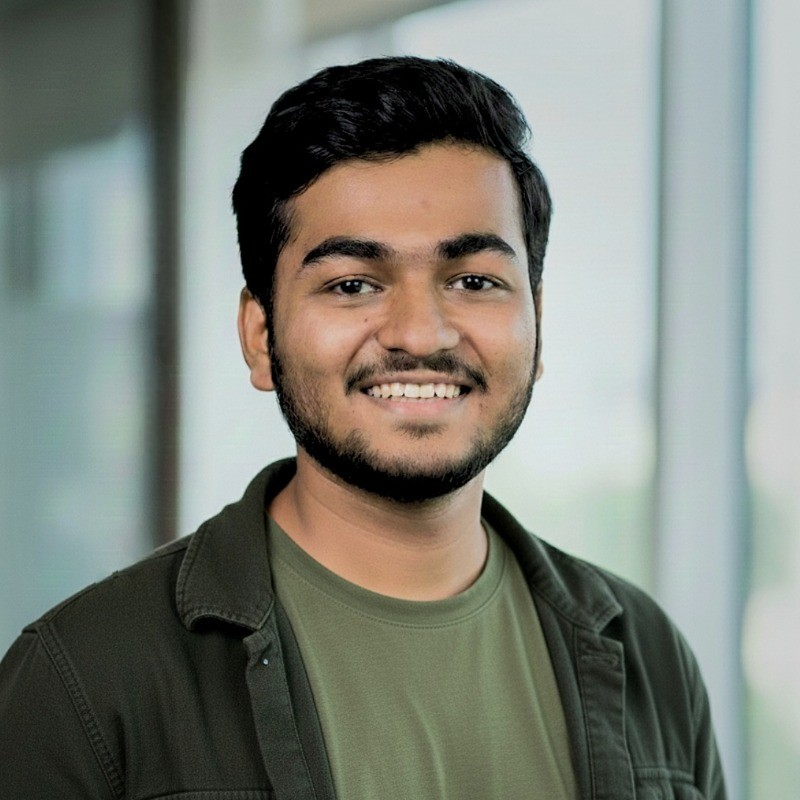
\includegraphics[width=3cm]{../../shivsarwade.jpg}
\end{minipage}

\vspace{5pt}


\section*{Technical Skills}
\textbf{Skilled:}\\[2pt]
HTML, CSS, Tailwind CSS, Node.js, Express.js, React.js, Next.js, RESTful APIs, JavaScript (ES6+), PostgreSQL, Git, UI/UX,  RBAC, Postman, JWT

\vspace{4pt}
\textbf{Intermediate:}\\[2pt]
Python, Java, AWS, MongoDB, DSA, System Design, Microservices, Mono Repo, Monolithic Architecture   

\vspace{4pt}
\textbf{Basic:}\\[2pt]
Redis, Nginx, Docker, RAG, LangGraph, Vercel, Supabase,
CI/CD.\section*{Projects}

\textbf{Griffion -- Identity \& Authentication Service}\\
\textbf{Synopsis:} Developed a modular authentication microservice serving as the core identity provider for internal tools. My personal contribution involved architecting the backend systems, building secure REST APIs, designing database schemas, and setting up protected frontend routing using \textbf{Node.js, React.js, MongoDB, Redis, and JWT}. \textbf{Challenge \& Independent Research:} A major challenge was high authorization latency under concurrent requests. Through independent research into database optimization and caching layers, I implemented efficient indexing and Redis caching strategies, successfully reducing query overhead and authorization latency by 30\%.

\vspace{6pt}

\textbf{JobJet -- Full-Stack Job Portal}\\
\textbf{Synopsis:} Engineered a scalable job-matching platform facilitating seamless recruiter-candidate interactions. I solely developed the backend infrastructure for application tracking, secure resume uploads, and user profile management, along with building a responsive component-driven frontend using \textbf{React.js, Node.js, MongoDB and Tailwind CSS}. \textbf{Challenge \& Independent Research:} A significant challenge was matching candidates to jobs from large datasets efficiently. I solved this by independently researching and implementing an optimized string search and sorting algorithm in Python to handle the data load effectively.

\vspace{6pt}

\textbf{TICKETIFY -- Event Management System}\\
\textbf{Synopsis:} Engineered a cross-platform event application backend supporting high-concurrency ticket booking and real-time attendee synchronization. My contribution focused on creating highly available REST APIs and implementing secure QR-based ticket validation for reliable check-ins using \textbf{React Native, Node.js, and MongoDB}. \textbf{Challenge \& Independent Research:} I faced challenges handling high concurrency under heavy load during ticket sales. I addressed this by independently researching distributed system patterns and implementing fault-tolerant asynchronous services to prevent system bottlenecks.

\section*{Experience}
\textbf{Software Developer} $|$ \textit{Sitramix, Pune} \hfill May 2025 -- June 2026\\
\vspace{-6pt}
\begin{itemize}[leftmargin=*]
    \item Developed responsive and interactive frontend interfaces, contributing to the deployment of production-ready pages across 4 major projects.
    \item Architected scalable backend systems, optimizing RESTful API endpoints (reducing response time by 40\%) and implementing robust JWT/RBAC security.
    \item Managed cloud infrastructure and deployment pipelines on AWS EC2 and S3, ensuring 99.9\% system uptime.
\end{itemize}

\vspace{6pt}

\textbf{GCC Social Member} $|$ \textit{Garware College of Commerce} \hfill August 2023 -- May 2025\\
\vspace{-6pt}
\begin{itemize}[leftmargin=*]
    \item Worked as a Social Media Executive managing digital operations and content strategy.
    \item Handled professional platforms including LinkedIn to drive audience engagement.
\end{itemize}

\vspace{6pt}

\textbf{Digital Marketing Intern} $|$ \textit{Garware College of Commerce, Pune} \hfill April 2024 -- June 2024\\
\vspace{-6pt}
\begin{itemize}[leftmargin=*]
    \item Contributed to digital marketing campaigns for college drives across YouTube, Instagram, and LinkedIn.
    \item Focused on user engagement, audience targeting, and content strategy.
\end{itemize}

\section*{Education}
\textbf{Master of Computer Applications (MCA)} $|$ \textit{Savitribai Phule Pune University} \hfill Expected: June 2027 \quad \textbf{CGPA: 8.93} \textbf{(81.80\%)}

\vspace{4pt} 

\textbf{Bachelor of Business Administration in Computer Applications (BBACA)} $|$ \textit{SPPU} \hfill 2025 \quad \textbf{CGPA: 9.60} \textbf{(92\%)} \quad \textbf{(1st Rank)}

\vspace{4pt} 

\textbf{12th Class Higher Secondary Certification (H.S.C.)} \hfill 2021 -- 2022 \quad \textbf{Percentage: 87.50\%} \quad \textbf{(1st Rank)}

\vspace{4pt} 

\textbf{10th Class Secondary School Certification (S.S.C.)} \hfill 2019 -- 2020 \quad \textbf{Percentage: 88.20\%} \quad \textbf{(1st Rank)}

\end{document}
